\section{Experimente}
%
\subsection{Wahl der Spezifikationssprache}
%
%
\begin{frame}
	\frametitle{Überblick}
	\tableofcontents[currentsubsection]
\end{frame}
%
\begin{frame}
	\frametitle{Wahl der Spezifikationssprache (1)}
	Experiment von 1978-1983 \cite{Avizienis:1984:FTD:1319725.1320045}:
	\begin{itemize}
		\item Szenario: Flughafenverwaltung
		\item Spezifikation in OBJ, PDL und Englisch geschrieben
		\item 18 Versionen in PL/1 implementiert
		\item 7 OBJ, 5 PDL und 6 englische Versionen
		\item PDL-Spezifikation mit 74 Seiten vs. 13 bei der OBJ- und 10 bei der englischen Spezifikation
	\end{itemize}
	
\end{frame}
%
%
\begin{frame}
	\frametitle{Wahl der Spezifikationssprache (2)}
	Durchführung des Experiments mit 100 Testtransaktionen:
	\begin{itemize}
		\item Transaktionsendpunkte als Vergleichsstellen
		\item 18-facher Vergleichsalgorithmus zur Ermittlung der korrekten Ergebnisse
		\item 816 Tripel-Kombinationen der Versionen getestet
	\end{itemize}	
\end{frame}
%
%
\begin{frame}
	\frametitle{Wahl der Spezifikationssprache (3)}
	Beobachtungen:
	\begin{itemize}
	\item Reine PDL-Tripel leicht zuverlässiger
	\item Jedoch kein gravierender Unterschied bezüglich der Spezifikationssprachen
	\item Mangelnde Präzision und Ausdrucksmöglichkeiten der untersuchten Sprachen
	\item Fehlinterpretationen der Spezifikationen
	\item Unabhängige Fehlerursachen führten häufig zu den selben falschen Ergebnissen.
	\end{itemize}	
\end{frame}
%
%
\subsection{Unabhängigkeit der Fehler}
%
\begin{frame}
	\frametitle{Überblick}
	\tableofcontents[currentsubsection]
\end{frame}
%
\begin{frame}
	\frametitle{Unabhängigkeit der Fehler}
	\begin{itemize}
		\item Annahme der N-Version Programmierung:
			\begin{itemize}
				\item Unabhängige Entwicklungskonditionen führen zu unabhängigen Fehlern in den einzelnen Versionen.
				\item Verschiedene Versionen versagen unabhängig voneinander.
				\item Zuverlässigkeit des Gesamtsystems ist deutlich höher als die der einzelnen Versionen.
			\end{itemize}
			\pause
			\item Aber:
			\begin{itemize}
				\item Programmierer tendieren bei anspruchsvollen Aufgaben dazu die selben Fehler zu machen.
				\item Enorme zusätzliche Kosten in der Entwicklung multipler Versionen
				\item Lohnt sich der Aufwand?
				\item $\implies$ Annahme der Fehlerunabhängigkeit untersuchen
			\end{itemize}
		
	\end{itemize}
	
\end{frame}
%
%
\begin{frame}
	\frametitle{Knight \& Leveson Experiment (1)}

	 Experiment zur Überprüfung der Unabhängigkeit von Fehlern in Versionen \cite{Knight:1986:EEA:10677.10688}:
		\begin{itemize}
			\item Raketenabwehrsystem als Zielprogramm
			\item 27 Versionen in Pascal auf Basis einer Spezifikation
			\item 241 Bit Vergleichsvektoren
			\item 1 Millionen automatisch generierte Testfälle
			\item Existierendes \enquote{\emph{Goldprogramm}} als Vergleichsmaßstab
			\item Doktoranden und Studenten der University of Virginia und der University of California
		\end{itemize}

\end{frame}
%
%
\begin{frame}
	\frametitle{ Knight \& Leveson Experiment(2)}
	
	Ergebnisse:
	\begin{itemize}
		\item Hohe Zuverlässigkeit in allen Versionen ($\geq 99\%$)
		\item Trotzdem hohes Auftreten gemeinsamer Fehler in Testfällen
		\item In 1255 Fällen versagte mehr als eine Version
		\item In 2 Fällen versagten sogar 8 Versionen
		\item Mehr gemeinsame Fehler aufgetreten, als bei eine Normalverteilung von unabhängigen Fehlern anzunehmen wäre
		\item Fehler aufgrund von mangelhaften mathematischen Kenntnissen
		\item Annahme der Fehlerunabhängigkeit zurückgewiesen
	\end{itemize}
	\pause
	
	Auf die nachfolgende Kritik des Experiments reagierten Knight und Leveson mit einer umfangreichen Antwort \cite{reply_critics}.
	
\end{frame}

\subsection{Aktuelle Forschungsprojekte}
%
%
\begin{frame}
	\frametitle{Überblick}
	\tableofcontents[currentsubsection]
\end{frame}
%
\begin{frame}
	\frametitle{Aktuelle Forschungsprojekte}
	
	\center{\huge{Wie geht's weiter?}}
	
\end{frame}
%
%
\begin{frame}
	\frametitle{Cloud-basierte Antiviren-Software}
	
	CloudAV, Antiviren-System als Netzwerk-Service in der Cloud \cite{Oberheide:2008:CNA:1496711.1496718}: 
	\begin{itemize}
		\item 10 verschiedene Viren-Erkennungssysteme
		\item $35\%$ höhere Erkennungsrate als herkömmliche Systeme bei aktuellen Gefahren
	\end{itemize}
	\pause
	\begin{figure}
		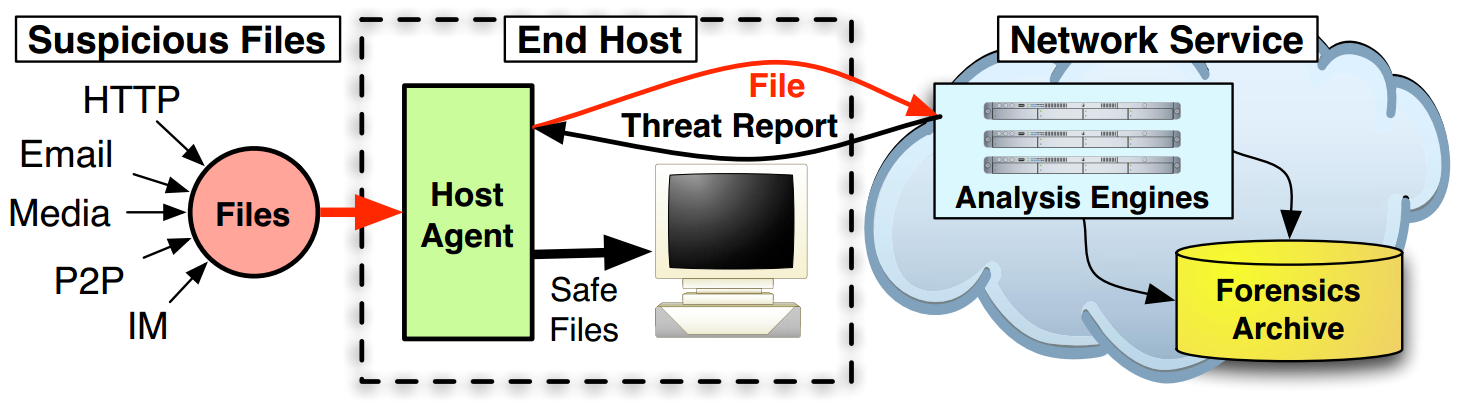
\includegraphics[scale=0.2]{grafiken/antivir.png}		
		\caption{Konzept CloudAV
			\footnotemark		
		}		
	\end{figure}
	\footnotetext{Quelle: \cite{Oberheide:2008:CNA:1496711.1496718}}
\end{frame}
%
%
\begin{frame}
	\frametitle{N-Version Website}

	\begin{itemize}
		\item 3 Versionen eines Online-Auktionshauses \cite{zero-day}
		\item Unterschiede in den Komponenten:
		\begin{itemize}
			\item Betriebssystem
			\item Webserver
			\item Programmiersprache
			\item DBMS
		\end{itemize}
		\item Ziel: Robustheit gegenüber Zero-Day-Exploits
		\item Schwachstelle: Verwaltender HTTP-Dispatcher

	\end{itemize}
	
\end{frame}
%